\documentclass[]{article}
\usepackage{lmodern}
\usepackage{amssymb,amsmath}
\usepackage{ifxetex,ifluatex}
\usepackage{fixltx2e} % provides \textsubscript
\ifnum 0\ifxetex 1\fi\ifluatex 1\fi=0 % if pdftex
  \usepackage[T1]{fontenc}
  \usepackage[utf8]{inputenc}
\else % if luatex or xelatex
  \ifxetex
    \usepackage{mathspec}
    \usepackage{xltxtra,xunicode}
  \else
    \usepackage{fontspec}
  \fi
  \defaultfontfeatures{Mapping=tex-text,Scale=MatchLowercase}
  \newcommand{\euro}{€}
\fi
% use upquote if available, for straight quotes in verbatim environments
\IfFileExists{upquote.sty}{\usepackage{upquote}}{}
% use microtype if available
\IfFileExists{microtype.sty}{%
\usepackage{microtype}
\UseMicrotypeSet[protrusion]{basicmath} % disable protrusion for tt fonts
}{}
\usepackage[margin=1in]{geometry}
\usepackage{graphicx}
\makeatletter
\def\maxwidth{\ifdim\Gin@nat@width>\linewidth\linewidth\else\Gin@nat@width\fi}
\def\maxheight{\ifdim\Gin@nat@height>\textheight\textheight\else\Gin@nat@height\fi}
\makeatother
% Scale images if necessary, so that they will not overflow the page
% margins by default, and it is still possible to overwrite the defaults
% using explicit options in \includegraphics[width, height, ...]{}
\setkeys{Gin}{width=\maxwidth,height=\maxheight,keepaspectratio}
\ifxetex
  \usepackage[setpagesize=false, % page size defined by xetex
              unicode=false, % unicode breaks when used with xetex
              xetex]{hyperref}
\else
  \usepackage[unicode=true]{hyperref}
\fi
\hypersetup{breaklinks=true,
            bookmarks=true,
            pdfauthor={FEDORU},
            pdftitle={Enquête logiciels SU - Septembre 2015},
            colorlinks=true,
            citecolor=blue,
            urlcolor=blue,
            linkcolor=magenta,
            pdfborder={0 0 0}}
\urlstyle{same}  % don't use monospace font for urls
\setlength{\parindent}{0pt}
\setlength{\parskip}{6pt plus 2pt minus 1pt}
\setlength{\emergencystretch}{3em}  % prevent overfull lines
\setcounter{secnumdepth}{5}

%%% Use protect on footnotes to avoid problems with footnotes in titles
\let\rmarkdownfootnote\footnote%
\def\footnote{\protect\rmarkdownfootnote}

%%% Change title format to be more compact
\usepackage{titling}

% Create subtitle command for use in maketitle
\newcommand{\subtitle}[1]{
  \posttitle{
    \begin{center}\large#1\end{center}
    }
}

\setlength{\droptitle}{-2em}
  \title{Enquête logiciels SU - Septembre 2015}
  \pretitle{\vspace{\droptitle}\centering\huge}
  \posttitle{\par}
  \author{FEDORU}
  \preauthor{\centering\large\emph}
  \postauthor{\par}
  \predate{\centering\large\emph}
  \postdate{\par}
  \date{07/09/2015}



\begin{document}

\maketitle


{
\hypersetup{linkcolor=black}
\setcounter{tocdepth}{2}
\tableofcontents
}
\section{7/9/2015}\label{section}

Reprise de l'exploitation des logiciels des SU

\begin{itemize}
\itemsep1pt\parskip0pt\parsep0pt
\item
  fichier source: DATA/FEDORU - ENQUETE LOGICIEL 2015 - V2 (12 06 15)
  (3)
\item
  création d'un dossier spécifique \textbf{Septembre2015} contenent un
  sous dossier \textbf{data} pour y stocker les résultats régionaux sous
  forme de fichier .csv.
\end{itemize}

\subsection{17/9/2015}\label{section-1}

\begin{itemize}
\itemsep1pt\parskip0pt\parsep0pt
\item
  récup données ORUMIP (Olivier Azema)
\end{itemize}

\subsection{Récupération des fichiers
csv}\label{recuperation-des-fichiers-csv}

\begin{itemize}
\itemsep1pt\parskip0pt\parsep0pt
\item
  les 5 premières lignes sont éliminées
\item
  élimination du héader =\textgreater{} il faudre en créer un
\end{itemize}

\begin{verbatim}
path = "./data/" # path = "./Septembre2015/data/" si console
out.file <- NULL
file.names <- dir(path, pattern =".csv") # seuls les fichiers se terminant par csv sont lus

for(i in 1:length(file.names)){
   file <- read.table(paste(path, file.names[i], sep=""), skip = 5, header = FALSE, sep=",", stringsAsFactors=FALSE)
   print(file.names[i])
   # on ne garde que les 22 premières colonnes
   file <- file[, 1:22]
   # on ne garde que les lignes où les colonnes 1 à 5 ne sont pas vides (http://genometoolbox.blogspot.fr/2014/01/remove-rows-with-na-values-from-r-data.html)
   file <- file[complete.cases(file[,1:5]),]
   # remplacement de la virgule écimale par le point décimal (soirce: http://stackoverflow.com/questions/5487164/r-how-to-replace-parts-of-variable-strings-within-data-frame)
   file <- as.data.frame(sapply(file, gsub, pattern = ",", replacement = "."))

   out.file <- rbind(out.file, file)
 }

n <- c("Region", "Departement", "FINESS", "Hopital", "CP", "Routage","Logiciel_2014","Editeur", "RPU_transmis","Nb_RPU_T1_2015", "Logiciel_2015", "Version_2015", "Coment", "Freq_remontee", "DN_exhaus","DN_confor", "DP_exhaus", "DP_confor", "MS_exhaus", "MS_confor", "Jours_manquants", "coment2")
 names(out.file) <- n

write.table(out.file, file = "archive.csv", sep=",", row.names = FALSE, qmethod = "double", fileEncoding="utf-8")
\end{verbatim}

\subsection{Récupération du fichier des
données}\label{recuperation-du-fichier-des-donnees}

\begin{itemize}
\itemsep1pt\parskip0pt\parsep0pt
\item
  Nombre de régions participantes: 9
\item
  Nombre de sites: 285
\end{itemize}

\section{Cartographie}\label{cartographie}

Cartographie des régions participantes et des logiciels.

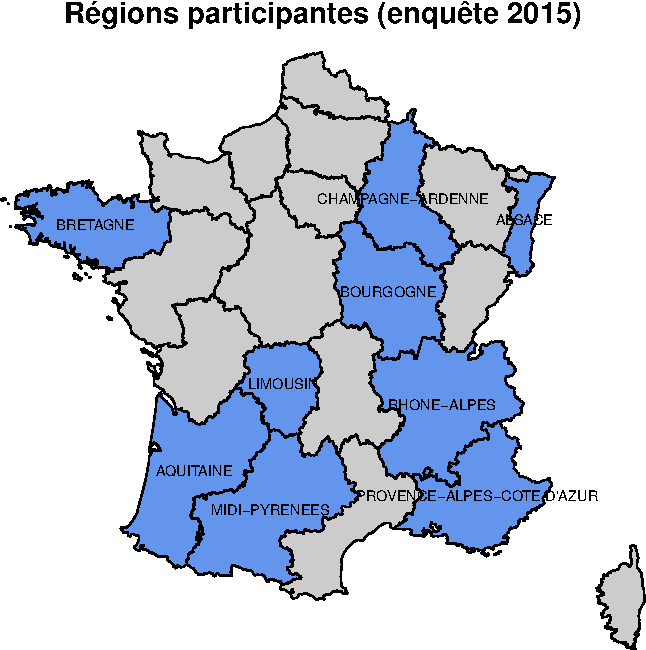
\includegraphics{septembre2015_files/figure-latex/carto_region-1.pdf}

\section{Editeurs}\label{editeurs}

\section{Logiciels 2015}\label{logiciels-2015}

\begin{itemize}
\itemsep1pt\parskip0pt\parsep0pt
\item
  Nombre de logiciels utilisés: 52
\end{itemize}

\subsection{Logiciels par ordre
décroissant}\label{logiciels-par-ordre-decroissant}

\begin{verbatim}

                   DMU             TU-ORUPACA                 URQUAL 
                    50                     45                     35 
           RESURGENCES                 DXCARE               CROSSWAY 
                    24                     13                     12 
              ATALANTE                  SIDSU       SILLAGE URGENCES 
                     9                      9                      8 
             MEDIBOARD                  ORBIS              POLYMEDIS 
                     7                      5                      5 
                 ORUV2               CLINICOM               DOPASOIN 
                     4                      3                      3 
         DOPA URGENCES                    DPU               EXPERTIZ 
                     3                      3                      3 
                SIGEMS ANTARES V2 DE INOVACUM               CORTEXTE 
                     3                      2                      2 
               EXAGONE        HOPITAL MANAGER        LOGICIEL MAISON 
                     2                      2                      2 
        MÉDICAL OBJECT                  OSOFT             RPUEXPRESS 
                     2                      2                      2 
               SANOCOM              SHAREGATE            SILLAGE DMU 
                     2                      2                      2 
           AGFA EXAGON                AXIGATE                 CLIMCO 
                     1                      1                      1 
          CORA URGENCE  DEVELOPPEMENT INTERNE                 DIAMMS 
                     1                      1                      1 
                  EMED               E SHERPA           EXPERT SANTE 
                     1                      1                      1 
          EXPERT SANTÉ                 MANUEL               MEDIBASE 
                     1                      1                      1 
              MEDINTUX                  MEDIS               MEDIWERE 
                     1                      1                      1 
                M-PLUS                 NAFAMA                 OSIRIS 
                     1                      1                      1 
                 QCARE                SPEC 4D             TRACK CARE 
                     1                      1                      1 
                URGEST 
                     1 
\end{verbatim}

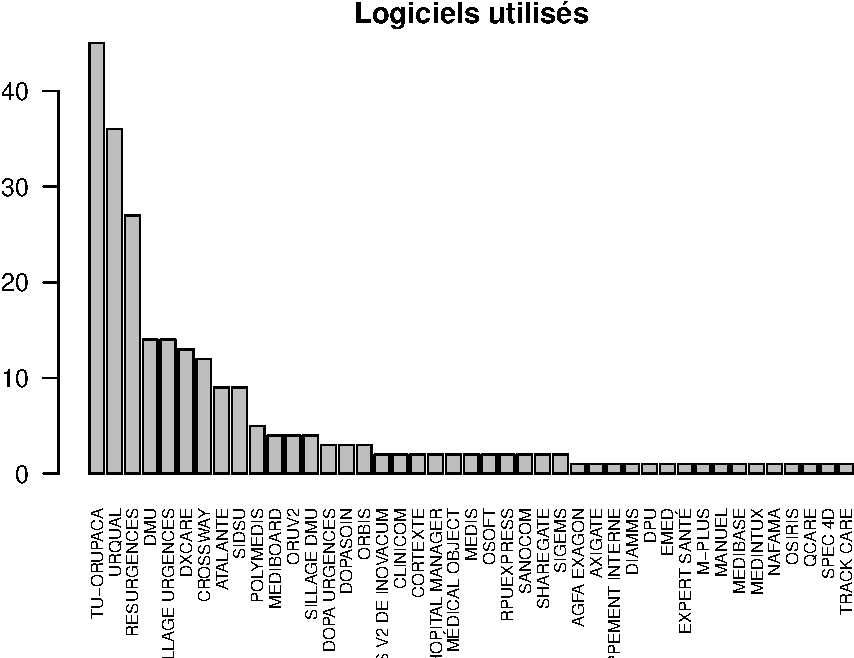
\includegraphics{septembre2015_files/figure-latex/unnamed-chunk-4-1.pdf}

\subsection{Logiciels par région}\label{logiciels-par-region}

\begin{verbatim}
                        
                         ALSACE AQUITAINE BOURGOGNE BRETAGNE
  AGFA EXAGON                 0         0         1        0
  ANTARES V2 DE INOVACUM      2         0         0        0
  ATALANTE                    8         0         1        0
  AXIGATE                     0         1         0        0
  CLIMCO                      0         0         0        0
  CLINICOM                    1         0         0        0
  CORA URGENCE                0         0         0        0
  CORTEXTE                    0         0         0        0
  CROSSWAY                    0         3         3        0
  DEVELOPPEMENT INTERNE       0         0         0        0
  DIAMMS                      0         0         0        0
  DMU                         2         0         7        0
  DOPASOIN                    0         0         0        0
  DOPA URGENCES               0         1         0        0
  DPU                         0         0         0        0
  DXCARE                      3         6         1        0
  EMED                        0         0         0        0
  E SHERPA                    0         0         0        0
  EXAGONE                     0         0         0        0
  EXPERTIZ                    0         0         0        0
  EXPERT SANTE                0         0         0        0
  EXPERT SANTÉ                0         0         0        0
  HOPITAL MANAGER             0         0         2        0
  LOGICIEL MAISON             0         0         0        0
  MANUEL                      0         0         1        0
  MEDIBASE                    0         1         0        0
  MEDIBOARD                   0         0         0        1
  MÉDICAL OBJECT              0         0         0        0
  MEDINTUX                    0         0         0        0
  MEDIS                       0         0         0        1
  MEDIWERE                    0         0         0        0
  M-PLUS                      0         1         0        0
  NAFAMA                      0         0         0        0
  ORBIS                       1         0         0        1
  ORUV2                       0         0         0        0
  OSIRIS                      0         0         0        0
  OSOFT                       0         0         0        1
  POLYMEDIS                   0         0         0        0
  QCARE                       0         0         0        0
  RESURGENCES                 1         1         3        7
  RPUEXPRESS                  0         0         0        0
  SANOCOM                     0         2         0        0
  SHAREGATE                   0         2         0        0
  SIDSU                       0         9         0        0
  SIGEMS                      0         2         0        0
  SILLAGE DMU                 0         0         0        2
  SILLAGE URGENCES            0         2         0        6
  SPEC 4D                     0         0         0        0
  TRACK CARE                  0         1         0        0
  TU-ORUPACA                  0         0         1        0
  URGEST                      0         0         0        0
  URQUAL                      0         3         3       11
                        
                         CHAMPAGNE ARDENNES LIMOUSIN MIDI PYRENEES PACA
  AGFA EXAGON                             0        0             0    0
  ANTARES V2 DE INOVACUM                  0        0             0    0
  ATALANTE                                0        0             0    0
  AXIGATE                                 0        0             0    0
  CLIMCO                                  0        0             0    0
  CLINICOM                                0        0             1    0
  CORA URGENCE                            0        0             0    0
  CORTEXTE                                0        0             2    0
  CROSSWAY                                0        0             6    0
  DEVELOPPEMENT INTERNE                   0        0             1    0
  DIAMMS                                  0        0             1    0
  DMU                                     3        0             0    2
  DOPASOIN                                0        0             3    0
  DOPA URGENCES                           2        0             0    0
  DPU                                     0        0             1    0
  DXCARE                                  1        0             2    0
  EMED                                    0        0             1    0
  E SHERPA                                0        0             0    0
  EXAGONE                                 0        0             0    0
  EXPERTIZ                                0        0             0    0
  EXPERT SANTE                            0        0             0    0
  EXPERT SANTÉ                            0        0             1    0
  HOPITAL MANAGER                         0        0             0    0
  LOGICIEL MAISON                         0        0             0    0
  MANUEL                                  0        0             0    0
  MEDIBASE                                0        0             0    0
  MEDIBOARD                               0        0             2    0
  MÉDICAL OBJECT                          0        0             2    0
  MEDINTUX                                0        0             0    1
  MEDIS                                   0        0             0    0
  MEDIWERE                                0        0             0    0
  M-PLUS                                  0        0             0    0
  NAFAMA                                  1        0             0    0
  ORBIS                                   0        0             0    0
  ORUV2                                   0        0             4    0
  OSIRIS                                  0        0             1    0
  OSOFT                                   0        0             0    0
  POLYMEDIS                               5        0             0    0
  QCARE                                   0        0             0    1
  RESURGENCES                             1        6             0    2
  RPUEXPRESS                              0        0             2    0
  SANOCOM                                 0        0             0    0
  SHAREGATE                               0        0             0    0
  SIDSU                                   0        0             0    0
  SIGEMS                                  0        0             0    0
  SILLAGE DMU                             0        0             0    0
  SILLAGE URGENCES                        0        0             0    0
  SPEC 4D                                 0        1             0    0
  TRACK CARE                              0        0             0    0
  TU-ORUPACA                              0        0             2   42
  URGEST                                  0        0             0    0
  URQUAL                                  3        2             5    2
                        
                         RHONE ALPES
  AGFA EXAGON                      0
  ANTARES V2 DE INOVACUM           0
  ATALANTE                         0
  AXIGATE                          0
  CLIMCO                           1
  CLINICOM                         1
  CORA URGENCE                     1
  CORTEXTE                         0
  CROSSWAY                         0
  DEVELOPPEMENT INTERNE            0
  DIAMMS                           0
  DMU                             36
  DOPASOIN                         0
  DOPA URGENCES                    0
  DPU                              2
  DXCARE                           0
  EMED                             0
  E SHERPA                         1
  EXAGONE                          2
  EXPERTIZ                         3
  EXPERT SANTE                     1
  EXPERT SANTÉ                     0
  HOPITAL MANAGER                  0
  LOGICIEL MAISON                  2
  MANUEL                           0
  MEDIBASE                         0
  MEDIBOARD                        4
  MÉDICAL OBJECT                   0
  MEDINTUX                         0
  MEDIS                            0
  MEDIWERE                         1
  M-PLUS                           0
  NAFAMA                           0
  ORBIS                            3
  ORUV2                            0
  OSIRIS                           0
  OSOFT                            1
  POLYMEDIS                        0
  QCARE                            0
  RESURGENCES                      3
  RPUEXPRESS                       0
  SANOCOM                          0
  SHAREGATE                        0
  SIDSU                            0
  SIGEMS                           1
  SILLAGE DMU                      0
  SILLAGE URGENCES                 0
  SPEC 4D                          0
  TRACK CARE                       0
  TU-ORUPACA                       0
  URGEST                           1
  URQUAL                           6
\end{verbatim}

Nombre de logiciels différents par région

\begin{verbatim}
            ALSACE          AQUITAINE          BOURGOGNE 
                 7                 14                 10 
          BRETAGNE CHAMPAGNE ARDENNES           LIMOUSIN 
                 8                  7                  3 
     MIDI PYRENEES               PACA        RHONE ALPES 
                17                  6                 18 
\end{verbatim}

\subsection{Cartographie des
logiciels}\label{cartographie-des-logiciels}

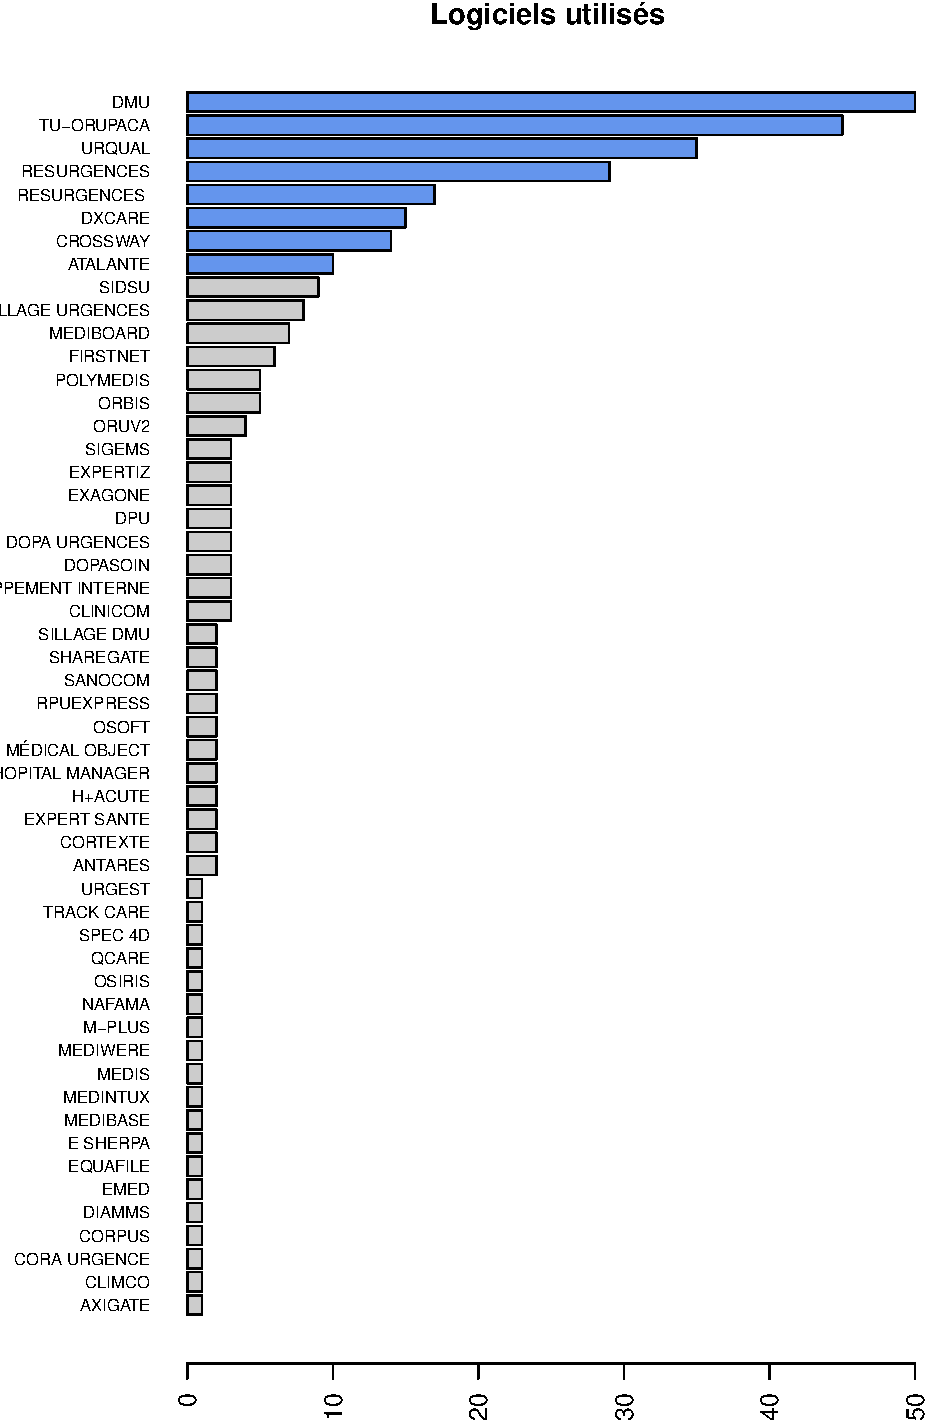
\includegraphics{septembre2015_files/figure-latex/unnamed-chunk-7-1.pdf}
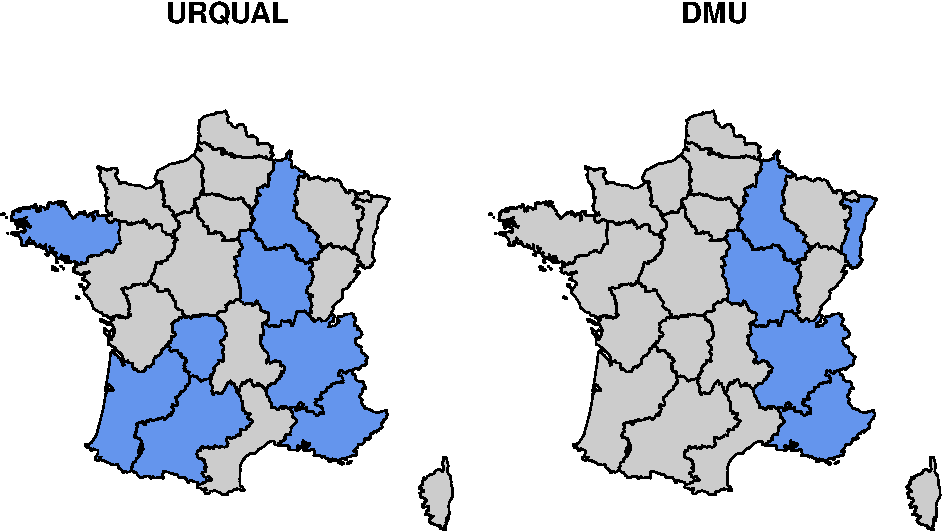
\includegraphics{septembre2015_files/figure-latex/unnamed-chunk-7-2.pdf}
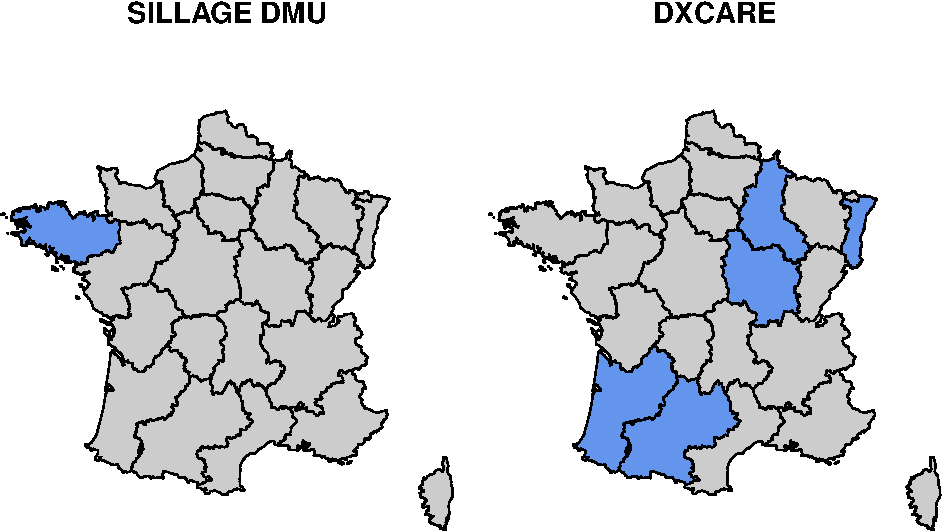
\includegraphics{septembre2015_files/figure-latex/unnamed-chunk-7-3.pdf}
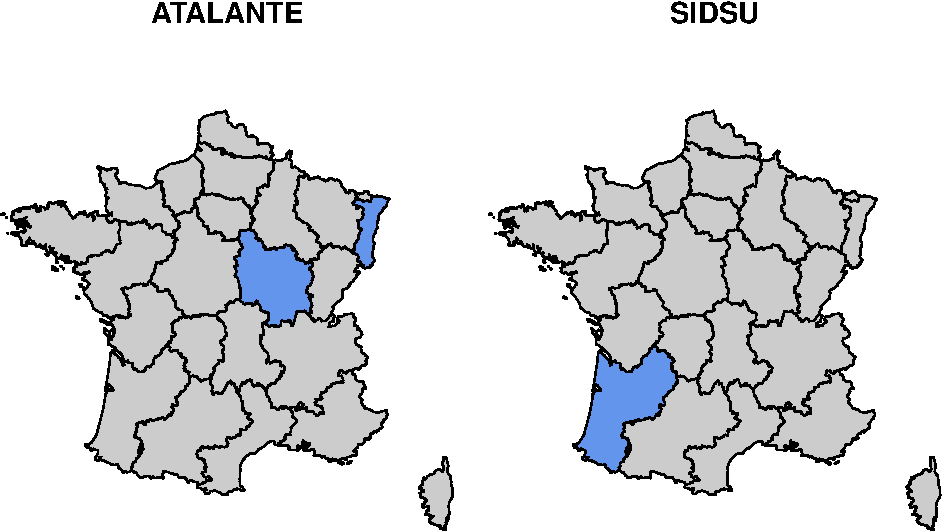
\includegraphics{septembre2015_files/figure-latex/unnamed-chunk-7-4.pdf}

\subsection{Un logiciel est présent dans combien de régions
?}\label{un-logiciel-est-present-dans-combien-de-regions}

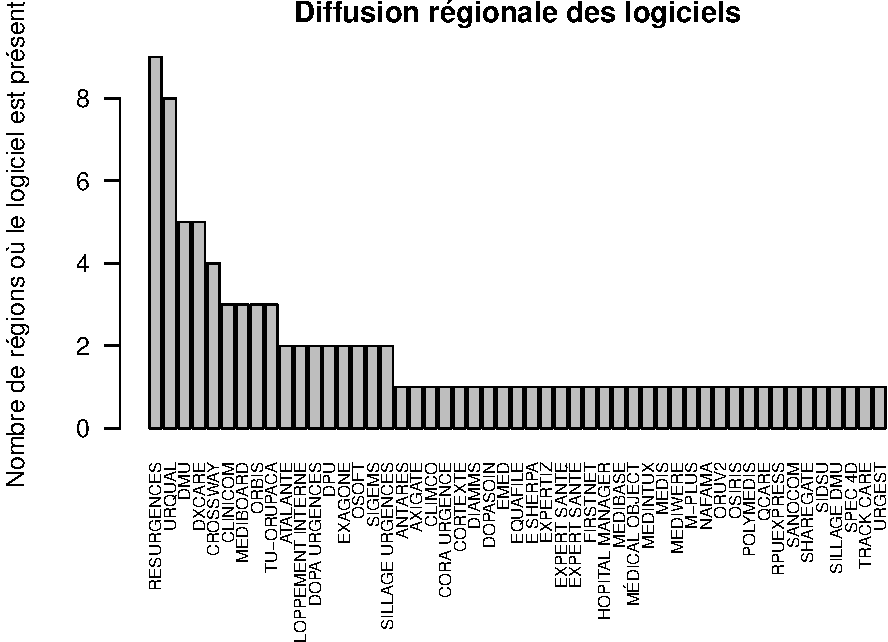
\includegraphics{septembre2015_files/figure-latex/unnamed-chunk-8-1.pdf}

\section{Analyse des RPU}\label{analyse-des-rpu}

Nombre de RPU produits: 1857473

\subsection{Nombre de RPU par
logiciel}\label{nombre-de-rpu-par-logiciel}

\begin{verbatim}
                       Nb de RPU
TU-ORUPACA                362364
URQUAL                    331497
DMU                       310522
RESURGENCES               181020
DXCARE                     97207
CROSSWAY                   60207
ATALANTE                   44712
SIDSU                      44401
DPU                        39714
MEDIBOARD                  33968
SILLAGE URGENCES           32519
POLYMEDIS                  20363
CLINICOM                   17623
EXPERTIZ                   15215
LOGICIEL MAISON            13956
MÉDICAL OBJECT             12577
CORTEXTE                   12369
SILLAGE DMU                11801
EXAGONE                    11463
TRACK CARE                 11345
ORUV2                      10715
ORBIS                      10669
DOPA URGENCES              10420
M-PLUS                      9970
DOPASOIN                    9329
ANTARES V2 DE INOVACUM      8974
SHAREGATE                   8639
CLIMCO                      8565
SIGEMS                      7231
SANOCOM                     7150
EXPERT SANTÉ                7058
OSOFT                       7050
SPEC 4D                     7015
MEDIS                       6974
CORA URGENCE                6618
EXPERT SANTE                6324
URGEST                      6321
MEDINTUX                    6224
MEDIWERE                    5676
RPUEXPRESS                  5205
NAFAMA                      5156
QCARE                       5131
AXIGATE                     4282
E SHERPA                    4090
MEDIBASE                    2913
HOPITAL MANAGER             2644
AGFA EXAGON                 2541
MANUEL                      2504
OSIRIS                      2019
DIAMMS                      1833
DEVELOPPEMENT INTERNE       1767
EMED                        1623
\end{verbatim}

\subsection{Nombre de jours manquants}\label{nombre-de-jours-manquants}

\subsubsection{Par logiciel}\label{par-logiciel}

\begin{verbatim}
                       Nb de jours manquants
URQUAL                                   116
TU-ORUPACA                                90
CROSSWAY                                  63
DOPASOIN                                  59
EMED                                      50
SILLAGE URGENCES                          42
ORBIS                                     30
OSOFT                                     21
DMU                                       20
LOGICIEL MAISON                           17
DPU                                        9
RESURGENCES                                5
CLINICOM                                   4
HOPITAL MANAGER                            3
MEDIBOARD                                  3
ATALANTE                                   2
E SHERPA                                   2
ANTARES V2 DE INOVACUM                     1
AGFA EXAGON                                0
AXIGATE                                    0
CLIMCO                                     0
CORA URGENCE                               0
CORTEXTE                                   0
DEVELOPPEMENT INTERNE                      0
DIAMMS                                     0
DOPA URGENCES                              0
DXCARE                                     0
EXAGONE                                    0
EXPERTIZ                                   0
EXPERT SANTE                               0
EXPERT SANTÉ                               0
MANUEL                                     0
MEDIBASE                                   0
MÉDICAL OBJECT                             0
MEDINTUX                                   0
MEDIS                                      0
MEDIWERE                                   0
M-PLUS                                     0
NAFAMA                                     0
ORUV2                                      0
OSIRIS                                     0
POLYMEDIS                                  0
QCARE                                      0
RPUEXPRESS                                 0
SANOCOM                                    0
SHAREGATE                                  0
SIDSU                                      0
SIGEMS                                     0
SILLAGE DMU                                0
SPEC 4D                                    0
TRACK CARE                                 0
URGEST                                     0
\end{verbatim}

\subsubsection{Par région}\label{par-region}

\begin{verbatim}
                   Nb de jours manquants
PACA                                 180
MIDI PYRENEES                        111
RHONE ALPES                           73
AQUITAINE                             63
BRETAGNE                              52
ALSACE                                34
BOURGOGNE                             21
CHAMPAGNE ARDENNES                     3
LIMOUSIN                               0
\end{verbatim}

\section{Indicateurs}\label{indicateurs}

Trois indicateurs ont été retenus:

\begin{itemize}
\itemsep1pt\parskip0pt\parsep0pt
\item
  Date de naissance
\item
  Diagnostic principal (DP)
\item
  Mode de sortie
\end{itemize}

Chaque indicateur a été évalué sur deux critères: \textbf{conformité} et
\textbf{exhaustivité}.

\subsection{Date de naissance}\label{date-de-naissance}

\begin{itemize}
\itemsep1pt\parskip0pt\parsep0pt
\item
  taux de conformité:
\end{itemize}

\begin{verbatim}
   Min. 1st Qu.  Median    Mean 3rd Qu.    Max.    NA's 
   0.00  100.00  100.00   99.64  100.00  100.00       7 
\end{verbatim}

\begin{itemize}
\itemsep1pt\parskip0pt\parsep0pt
\item
  conformité par outil:
\end{itemize}

\begin{verbatim}
                          Min    Max   moyenne   ecart-type Nb
AGFA EXAGON            100.00 100.00 100.00000           NA  1
ANTARES V2 DE INOVACUM 100.00 100.00 100.00000  0.000000000  2
ATALANTE               100.00 100.00 100.00000  0.000000000  9
AXIGATE                100.00 100.00 100.00000           NA  1
CLIMCO                 100.00 100.00 100.00000           NA  1
CLINICOM               100.00 100.00 100.00000  0.000000000  3
CORA URGENCE           100.00 100.00 100.00000           NA  1
CORTEXTE               100.00 100.00 100.00000  0.000000000  2
CROSSWAY                99.98 100.00  99.99727  0.006466698 12
DEVELOPPEMENT INTERNE   99.94  99.94  99.94000           NA  1
DIAMMS                 100.00 100.00 100.00000           NA  1
DMU                    100.00 100.00 100.00000  0.000000000 50
DOPASOIN                99.96 100.00  99.97333  0.023094011  3
DOPA URGENCES          100.00 100.00 100.00000  0.000000000  3
DPU                    100.00 100.00 100.00000  0.000000000  3
DXCARE                 100.00 100.00 100.00000  0.000000000 13
EMED                   100.00 100.00 100.00000           NA  1
E SHERPA               100.00 100.00 100.00000           NA  1
EXAGONE                100.00 100.00 100.00000  0.000000000  2
EXPERTIZ               100.00 100.00 100.00000  0.000000000  3
EXPERT SANTE           100.00 100.00 100.00000           NA  1
EXPERT SANTÉ           100.00 100.00 100.00000           NA  1
HOPITAL MANAGER        100.00 100.00 100.00000  0.000000000  2
LOGICIEL MAISON        100.00 100.00 100.00000  0.000000000  2
MANUEL                 100.00 100.00 100.00000           NA  1
MEDIBASE               100.00 100.00 100.00000           NA  1
MEDIBOARD               99.98 100.00  99.99714  0.007559289  7
MÉDICAL OBJECT         100.00 100.00 100.00000  0.000000000  2
MEDINTUX                99.92  99.92  99.92000           NA  1
MEDIS                  100.00 100.00 100.00000           NA  1
MEDIWERE               100.00 100.00 100.00000           NA  1
M-PLUS                 100.00 100.00 100.00000           NA  1
NAFAMA                  99.80  99.80  99.80000           NA  1
ORBIS                  100.00 100.00 100.00000  0.000000000  5
ORUV2                   98.74 100.00  99.64750  0.607144958  4
OSIRIS                  99.90  99.90  99.90000           NA  1
OSOFT                  100.00 100.00 100.00000  0.000000000  2
POLYMEDIS              100.00 100.00 100.00000  0.000000000  5
QCARE                   99.98  99.98  99.98000           NA  1
RESURGENCES             99.95 100.00  99.99750  0.010320937 24
RPUEXPRESS              99.89 100.00  99.94500  0.077781746  2
SANOCOM                100.00 100.00 100.00000  0.000000000  2
SHAREGATE              100.00 100.00 100.00000  0.000000000  2
SIDSU                  100.00 100.00 100.00000  0.000000000  9
SIGEMS                 100.00 100.00 100.00000  0.000000000  3
SILLAGE DMU            100.00 100.00 100.00000  0.000000000  2
SILLAGE URGENCES       100.00 100.00 100.00000  0.000000000  8
SPEC 4D                100.00 100.00 100.00000           NA  1
TRACK CARE             100.00 100.00 100.00000           NA  1
TU-ORUPACA               0.00 100.00  97.77778 14.907119850 45
URGEST                 100.00 100.00 100.00000           NA  1
URQUAL                  99.80 100.00  99.99206  0.034534077 35
\end{verbatim}

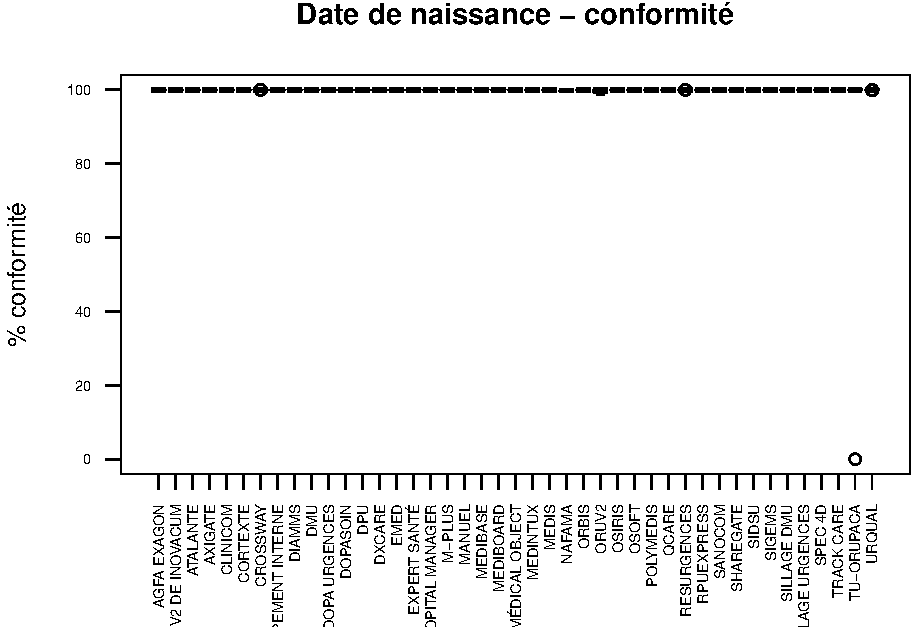
\includegraphics{septembre2015_files/figure-latex/unnamed-chunk-14-1.pdf}

\begin{itemize}
\itemsep1pt\parskip0pt\parsep0pt
\item
  taux d'exhaustivité:
\end{itemize}

\begin{verbatim}
   Min. 1st Qu.  Median    Mean 3rd Qu.    Max.    NA's 
   0.00  100.00  100.00   99.64  100.00  100.00       7 
\end{verbatim}

\begin{itemize}
\itemsep1pt\parskip0pt\parsep0pt
\item
  exhaustivité par outil
\end{itemize}

\begin{verbatim}
                          Min    Max   moyenne   ecart-type Nb
AGFA EXAGON            100.00 100.00 100.00000           NA  1
ANTARES V2 DE INOVACUM 100.00 100.00 100.00000  0.000000000  2
ATALANTE               100.00 100.00 100.00000  0.000000000  9
AXIGATE                100.00 100.00 100.00000           NA  1
CLIMCO                 100.00 100.00 100.00000           NA  1
CLINICOM               100.00 100.00 100.00000  0.000000000  3
CORA URGENCE           100.00 100.00 100.00000           NA  1
CORTEXTE               100.00 100.00 100.00000  0.000000000  2
CROSSWAY               100.00 100.00 100.00000  0.000000000 12
DEVELOPPEMENT INTERNE  100.00 100.00 100.00000           NA  1
DIAMMS                 100.00 100.00 100.00000           NA  1
DMU                    100.00 100.00 100.00000  0.000000000 50
DOPASOIN                99.96 100.00  99.97333  0.023094011  3
DOPA URGENCES          100.00 100.00 100.00000  0.000000000  3
DPU                    100.00 100.00 100.00000  0.000000000  3
DXCARE                 100.00 100.00 100.00000  0.000000000 13
EMED                   100.00 100.00 100.00000           NA  1
E SHERPA               100.00 100.00 100.00000           NA  1
EXAGONE                100.00 100.00 100.00000  0.000000000  2
EXPERTIZ               100.00 100.00 100.00000  0.000000000  3
EXPERT SANTE           100.00 100.00 100.00000           NA  1
EXPERT SANTÉ           100.00 100.00 100.00000           NA  1
HOPITAL MANAGER        100.00 100.00 100.00000  0.000000000  2
LOGICIEL MAISON        100.00 100.00 100.00000  0.000000000  2
MANUEL                 100.00 100.00 100.00000           NA  1
MEDIBASE               100.00 100.00 100.00000           NA  1
MEDIBOARD              100.00 100.00 100.00000  0.000000000  7
MÉDICAL OBJECT         100.00 100.00 100.00000  0.000000000  2
MEDINTUX                99.92  99.92  99.92000           NA  1
MEDIS                  100.00 100.00 100.00000           NA  1
MEDIWERE               100.00 100.00 100.00000           NA  1
M-PLUS                 100.00 100.00 100.00000           NA  1
NAFAMA                  99.80  99.80  99.80000           NA  1
ORBIS                  100.00 100.00 100.00000  0.000000000  5
ORUV2                   99.97 100.00  99.99250  0.015000000  4
OSIRIS                 100.00 100.00 100.00000           NA  1
OSOFT                  100.00 100.00 100.00000  0.000000000  2
POLYMEDIS              100.00 100.00 100.00000  0.000000000  5
QCARE                   99.98  99.98  99.98000           NA  1
RESURGENCES             99.95 100.00  99.99750  0.010320937 24
RPUEXPRESS             100.00 100.00 100.00000  0.000000000  2
SANOCOM                100.00 100.00 100.00000  0.000000000  2
SHAREGATE              100.00 100.00 100.00000  0.000000000  2
SIDSU                  100.00 100.00 100.00000  0.000000000  9
SIGEMS                 100.00 100.00 100.00000  0.000000000  3
SILLAGE DMU            100.00 100.00 100.00000  0.000000000  2
SILLAGE URGENCES       100.00 100.00 100.00000  0.000000000  8
SPEC 4D                100.00 100.00 100.00000           NA  1
TRACK CARE             100.00 100.00 100.00000           NA  1
TU-ORUPACA               0.00 100.00  97.77778 14.907119850 45
URGEST                 100.00 100.00 100.00000           NA  1
URQUAL                  99.99 100.00  99.99971  0.001714986 35
\end{verbatim}

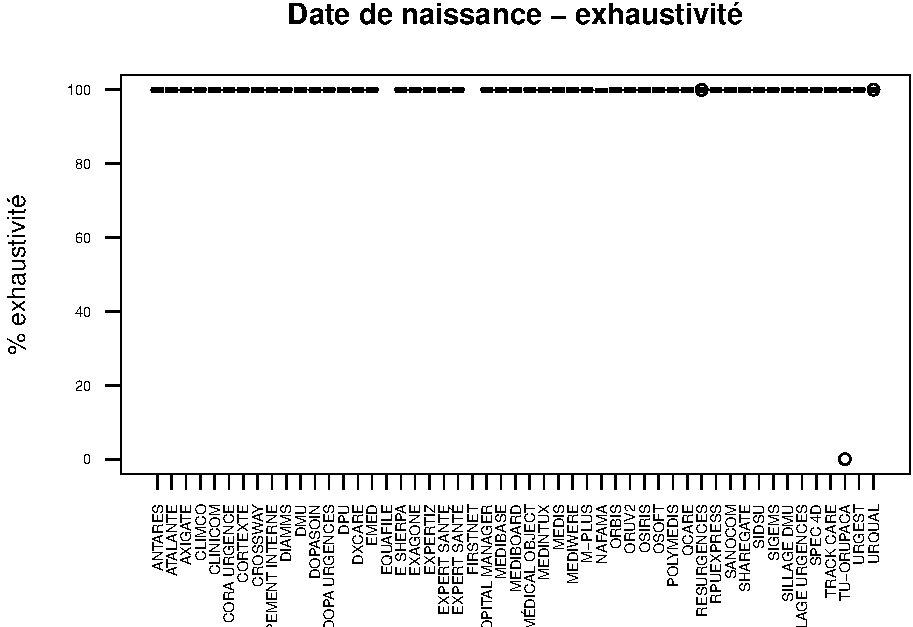
\includegraphics{septembre2015_files/figure-latex/unnamed-chunk-16-1.pdf}

\subsection{Diagnostic (DP)}\label{diagnostic-dp}

\begin{itemize}
\itemsep1pt\parskip0pt\parsep0pt
\item
  taux de conformité:
\end{itemize}

\begin{verbatim}
   Min. 1st Qu.  Median    Mean 3rd Qu.    Max.    NA's 
   0.00   76.00   95.00   76.82   97.57  100.00       7 
\end{verbatim}

\begin{itemize}
\itemsep1pt\parskip0pt\parsep0pt
\item
  conformité par outil
\end{itemize}

\begin{verbatim}
                          Min    Max   moyenne  ecart-type Nb
AGFA EXAGON             12.00  12.00  12.00000          NA  1
ANTARES V2 DE INOVACUM  45.84  90.51  68.17500 31.58645992  2
ATALANTE                 0.00  98.95  38.23222 35.61581102  9
AXIGATE                  0.00   0.00   0.00000          NA  1
CLIMCO                  95.00  95.00  95.00000          NA  1
CLINICOM                95.00  98.03  96.39000  1.53039211  3
CORA URGENCE            95.00  95.00  95.00000          NA  1
CORTEXTE                87.11  99.49  93.30000  8.75398195  2
CROSSWAY                 0.00 100.00  54.80636 42.90460238 12
DEVELOPPEMENT INTERNE  100.00 100.00 100.00000          NA  1
DIAMMS                  78.56  78.56  78.56000          NA  1
DMU                     56.80 100.00  93.83813  6.91259955 50
DOPASOIN                 0.00  97.49  32.49667 56.28587774  3
DOPA URGENCES            0.00  62.90  20.96667 36.31533193  3
DPU                     92.18  95.00  94.06000  1.62812776  3
DXCARE                   0.00  98.90  54.74923 35.50656429 13
EMED                    97.54  97.54  97.54000          NA  1
E SHERPA                95.00  95.00  95.00000          NA  1
EXAGONE                 95.00  95.00  95.00000  0.00000000  2
EXPERTIZ                95.00  95.00  95.00000  0.00000000  3
EXPERT SANTE            95.00  95.00  95.00000          NA  1
EXPERT SANTÉ            29.20  29.20  29.20000          NA  1
HOPITAL MANAGER         95.00 100.00  97.50000  3.53553391  2
LOGICIEL MAISON         95.00  95.00  95.00000  0.00000000  2
MANUEL                  98.00  98.00  98.00000          NA  1
MEDIBASE                96.40  96.40  96.40000          NA  1
MEDIBOARD                0.73  95.00  64.05857 40.50008083  7
MÉDICAL OBJECT          49.76  90.77  70.26500 28.99844910  2
MEDINTUX                92.15  92.15  92.15000          NA  1
MEDIS                   19.70  19.70  19.70000          NA  1
MEDIWERE                95.00  95.00  95.00000          NA  1
M-PLUS                  83.50  83.50  83.50000          NA  1
NAFAMA                  98.50  98.50  98.50000          NA  1
ORBIS                    0.00  95.00  31.66667 54.84827557  5
ORUV2                    0.00  98.90  58.10250 48.84531528  4
OSIRIS                 100.00 100.00 100.00000          NA  1
OSOFT                   95.00  98.60  96.80000  2.54558441  2
POLYMEDIS               97.40  99.70  98.50000  1.04403065  5
QCARE                    0.00   0.00   0.00000          NA  1
RESURGENCES             76.00 100.00  95.78750  5.34353103 24
RPUEXPRESS              87.22  91.95  89.58500  3.34461508  2
SANOCOM                 76.70  83.30  80.00000  4.66690476  2
SHAREGATE                0.00   0.10   0.05000  0.07071068  2
SIDSU                   27.30  99.80  87.05556 22.82515669  9
SIGEMS                   8.40  95.00  51.70000 61.23544725  3
SILLAGE DMU              0.90  10.50   5.70000  6.78822510  2
SILLAGE URGENCES         0.00  95.00  57.06250 42.86933428  8
SPEC 4D                 85.57  85.57  85.57000          NA  1
TRACK CARE              96.30  96.30  96.30000          NA  1
TU-ORUPACA               0.00  99.29  92.82267 15.63095899 45
URGEST                  95.00  95.00  95.00000          NA  1
URQUAL                   0.00 100.00  61.16588 43.18051175 35
\end{verbatim}

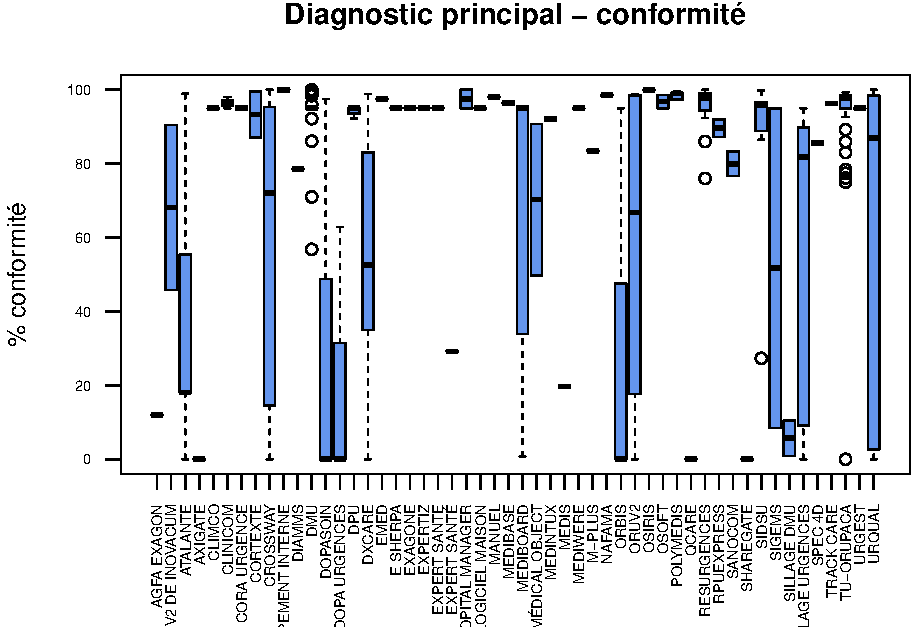
\includegraphics{septembre2015_files/figure-latex/unnamed-chunk-18-1.pdf}

\begin{itemize}
\itemsep1pt\parskip0pt\parsep0pt
\item
  taux de exhaustivité:
\end{itemize}

\begin{verbatim}
   Min. 1st Qu.  Median    Mean 3rd Qu.    Max.    NA's 
   0.00   55.40   93.79   72.35   98.11  100.00       7 
\end{verbatim}

\begin{itemize}
\itemsep1pt\parskip0pt\parsep0pt
\item
  exhaustivité par outil
\end{itemize}

\begin{verbatim}
                          Min    Max   moyenne  ecart-type Nb
AGFA EXAGON             12.00  12.00  12.00000          NA  1
ANTARES V2 DE INOVACUM  45.84  90.51  68.17500 31.58645992  2
ATALANTE                 0.00  98.95  38.23222 35.61581102  9
AXIGATE                  0.00   0.00   0.00000          NA  1
CLIMCO                  38.00  38.00  38.00000          NA  1
CLINICOM                72.00  98.03  88.72333 14.51362923  3
CORA URGENCE            95.00  95.00  95.00000          NA  1
CORTEXTE                87.57  99.52  93.54500  8.44992604  2
CROSSWAY                 0.00 100.00  54.81909 42.91168360 12
DEVELOPPEMENT INTERNE  100.00 100.00 100.00000          NA  1
DIAMMS                  78.72  78.72  78.72000          NA  1
DMU                      2.00 100.00  89.25833 16.70325683 50
DOPASOIN                 0.00  97.71  32.57000 56.41289480  3
DOPA URGENCES            0.00  62.90  20.96667 36.31533193  3
DPU                     87.00  97.00  92.06000  5.00107988  3
DXCARE                   0.00  98.90  54.74923 35.50656429 13
EMED                    97.60  97.60  97.60000          NA  1
E SHERPA                 0.00   0.00   0.00000          NA  1
EXAGONE                  0.00   4.00   2.00000  2.82842712  2
EXPERTIZ                82.00  94.00  88.66667  6.11010093  3
EXPERT SANTE            95.00  95.00  95.00000          NA  1
EXPERT SANTÉ            29.22  29.22  29.22000          NA  1
HOPITAL MANAGER         95.00 100.00  97.50000  3.53553391  2
LOGICIEL MAISON         83.00  95.00  89.00000  8.48528137  2
MANUEL                  99.00  99.00  99.00000          NA  1
MEDIBASE                96.40  96.40  96.40000          NA  1
MEDIBOARD                0.00  43.20  10.34429 16.96571824  7
MÉDICAL OBJECT          49.76  90.77  70.26500 28.99844910  2
MEDINTUX               100.00 100.00 100.00000          NA  1
MEDIS                   19.70  19.70  19.70000          NA  1
MEDIWERE               100.00 100.00 100.00000          NA  1
M-PLUS                  83.50  83.50  83.50000          NA  1
NAFAMA                  99.80  99.80  99.80000          NA  1
ORBIS                    0.00   0.00   0.00000  0.00000000  5
ORUV2                    0.00  98.90  58.18500 48.93563017  4
OSIRIS                 100.00 100.00 100.00000          NA  1
OSOFT                    0.00  98.60  49.30000 69.72072862  2
POLYMEDIS               97.40  99.70  98.74000  0.84734881  5
QCARE                    0.00   0.00   0.00000          NA  1
RESURGENCES             76.00 100.00  95.94583  5.30377299 24
RPUEXPRESS              87.22  91.95  89.58500  3.34461508  2
SANOCOM                 76.70  83.30  80.00000  4.66690476  2
SHAREGATE                0.00   0.10   0.05000  0.07071068  2
SIDSU                   27.30  99.80  87.05556 22.82515669  9
SIGEMS                   8.40  80.00  44.20000 50.62884553  3
SILLAGE DMU              0.90  10.50   5.70000  6.78822510  2
SILLAGE URGENCES         0.00  95.00  57.06250 42.86933428  8
SPEC 4D                 85.57  85.57  85.57000          NA  1
TRACK CARE              96.30  96.30  96.30000          NA  1
TU-ORUPACA               0.00  99.29  92.83622 15.63379909 45
URGEST                  98.00  98.00  98.00000          NA  1
URQUAL                   0.00 100.00  58.69941 42.77801580 35
\end{verbatim}

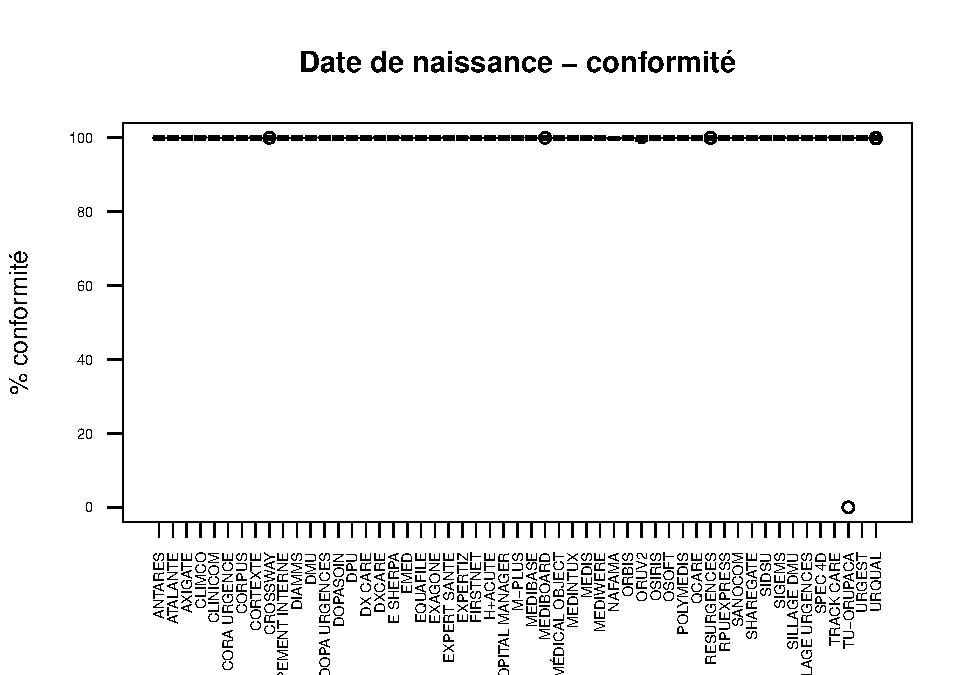
\includegraphics{septembre2015_files/figure-latex/unnamed-chunk-20-1.pdf}

\subsection{Mode de sortie (MS)}\label{mode-de-sortie-ms}

\begin{itemize}
\itemsep1pt\parskip0pt\parsep0pt
\item
  taux de conformité:
\end{itemize}

\begin{verbatim}
   Min. 1st Qu.  Median    Mean 3rd Qu.    Max.    NA's 
   0.00   93.77   99.52   87.59   99.98  100.00      72 
\end{verbatim}

\begin{itemize}
\itemsep1pt\parskip0pt\parsep0pt
\item
  conformité par outil
\end{itemize}

\begin{verbatim}
Warning in FUN(X[[i]], ...): aucun argument trouvé pour min ; Inf est
renvoyé
\end{verbatim}

\begin{verbatim}
Warning in FUN(X[[i]], ...): aucun argument trouvé pour min ; Inf est
renvoyé
\end{verbatim}

\begin{verbatim}
Warning in FUN(X[[i]], ...): aucun argument trouvé pour min ; Inf est
renvoyé
\end{verbatim}

\begin{verbatim}
Warning in FUN(X[[i]], ...): aucun argument trouvé pour min ; Inf est
renvoyé
\end{verbatim}

\begin{verbatim}
Warning in FUN(X[[i]], ...): aucun argument trouvé pour min ; Inf est
renvoyé
\end{verbatim}

\begin{verbatim}
Warning in FUN(X[[i]], ...): aucun argument trouvé pour min ; Inf est
renvoyé
\end{verbatim}

\begin{verbatim}
Warning in FUN(X[[i]], ...): aucun argument trouvé pour min ; Inf est
renvoyé
\end{verbatim}

\begin{verbatim}
Warning in FUN(X[[i]], ...): aucun argument trouvé pour min ; Inf est
renvoyé
\end{verbatim}

\begin{verbatim}
Warning in FUN(X[[i]], ...): aucun argument trouvé pour min ; Inf est
renvoyé
\end{verbatim}

\begin{verbatim}
Warning in FUN(X[[i]], ...): aucun argument pour max ; -Inf est renvoyé
\end{verbatim}

\begin{verbatim}
Warning in FUN(X[[i]], ...): aucun argument pour max ; -Inf est renvoyé
\end{verbatim}

\begin{verbatim}
Warning in FUN(X[[i]], ...): aucun argument pour max ; -Inf est renvoyé
\end{verbatim}

\begin{verbatim}
Warning in FUN(X[[i]], ...): aucun argument pour max ; -Inf est renvoyé
\end{verbatim}

\begin{verbatim}
Warning in FUN(X[[i]], ...): aucun argument pour max ; -Inf est renvoyé
\end{verbatim}

\begin{verbatim}
Warning in FUN(X[[i]], ...): aucun argument pour max ; -Inf est renvoyé
\end{verbatim}

\begin{verbatim}
Warning in FUN(X[[i]], ...): aucun argument pour max ; -Inf est renvoyé
\end{verbatim}

\begin{verbatim}
Warning in FUN(X[[i]], ...): aucun argument pour max ; -Inf est renvoyé
\end{verbatim}

\begin{verbatim}
Warning in FUN(X[[i]], ...): aucun argument pour max ; -Inf est renvoyé
\end{verbatim}

\begin{verbatim}
                          Min    Max   moyenne ecart-type Nb
AGFA EXAGON            100.00 100.00 100.00000         NA  1
ANTARES V2 DE INOVACUM  83.99  84.48  84.23500  0.3464823  2
ATALANTE                 0.00  99.14  59.77889 37.0790394  9
AXIGATE                 99.90  99.90  99.90000         NA  1
CLIMCO                    Inf   -Inf       NaN         NA  1
CLINICOM                98.66 100.00  99.33000  0.9475231  3
CORA URGENCE              Inf   -Inf       NaN         NA  1
CORTEXTE                99.43  99.70  99.56500  0.1909188  2
CROSSWAY                 0.00  99.44  49.59364 47.9639632 12
DEVELOPPEMENT INTERNE   99.89  99.89  99.89000         NA  1
DIAMMS                  80.47  80.47  80.47000         NA  1
DMU                     97.41 100.00  99.39071  1.0119096 50
DOPASOIN                72.48  86.54  78.59333  7.2070614  3
DOPA URGENCES           69.10  82.60  77.36667  7.2431577  3
DPU                     99.76  99.76  99.76000         NA  3
DXCARE                  21.05 100.00  86.82538 29.3565517 13
EMED                   100.00 100.00 100.00000         NA  1
E SHERPA                  Inf   -Inf       NaN         NA  1
EXAGONE                   Inf   -Inf       NaN         NA  2
EXPERTIZ                  Inf   -Inf       NaN         NA  3
EXPERT SANTE              Inf   -Inf       NaN         NA  1
EXPERT SANTÉ            99.93  99.93  99.93000         NA  1
HOPITAL MANAGER        100.00 100.00 100.00000  0.0000000  2
LOGICIEL MAISON           Inf   -Inf       NaN         NA  2
MANUEL                  99.00  99.00  99.00000         NA  1
MEDIBASE                65.70  65.70  65.70000         NA  1
MEDIBOARD               99.53  99.96  99.81333  0.2454248  7
MÉDICAL OBJECT          49.52  90.67  70.09500 29.0974440  2
MEDINTUX               100.00 100.00 100.00000         NA  1
MEDIS                   13.50  13.50  13.50000         NA  1
MEDIWERE                  Inf   -Inf       NaN         NA  1
M-PLUS                  16.80  16.80  16.80000         NA  1
NAFAMA                  99.80  99.80  99.80000         NA  1
ORBIS                   15.70  19.80  17.75000  2.8991378  5
ORUV2                   39.45  99.92  84.27000 29.8845211  4
OSIRIS                 100.00 100.00 100.00000         NA  1
OSOFT                  100.00 100.00 100.00000         NA  2
POLYMEDIS               99.30  99.90  99.68000  0.2683282  5
QCARE                    0.00   0.00   0.00000         NA  1
RESURGENCES              0.00 100.00  85.14286 35.6807092 24
RPUEXPRESS              93.58  94.01  93.79500  0.3040559  2
SANOCOM                100.00 100.00 100.00000  0.0000000  2
SHAREGATE              100.00 100.00 100.00000  0.0000000  2
SIDSU                   98.20 100.00  99.45556  0.5659309  9
SIGEMS                  99.90  99.90  99.90000         NA  3
SILLAGE DMU             98.80 100.00  99.40000  0.8485281  2
SILLAGE URGENCES        68.50  99.90  94.37500 10.7763962  8
SPEC 4D                 99.97  99.97  99.97000         NA  1
TRACK CARE              98.30  98.30  98.30000         NA  1
TU-ORUPACA               0.00 100.00  94.65756 15.6655159 45
URGEST                    Inf   -Inf       NaN         NA  1
URQUAL                  14.29 100.00  93.60621 16.4486166 35
\end{verbatim}

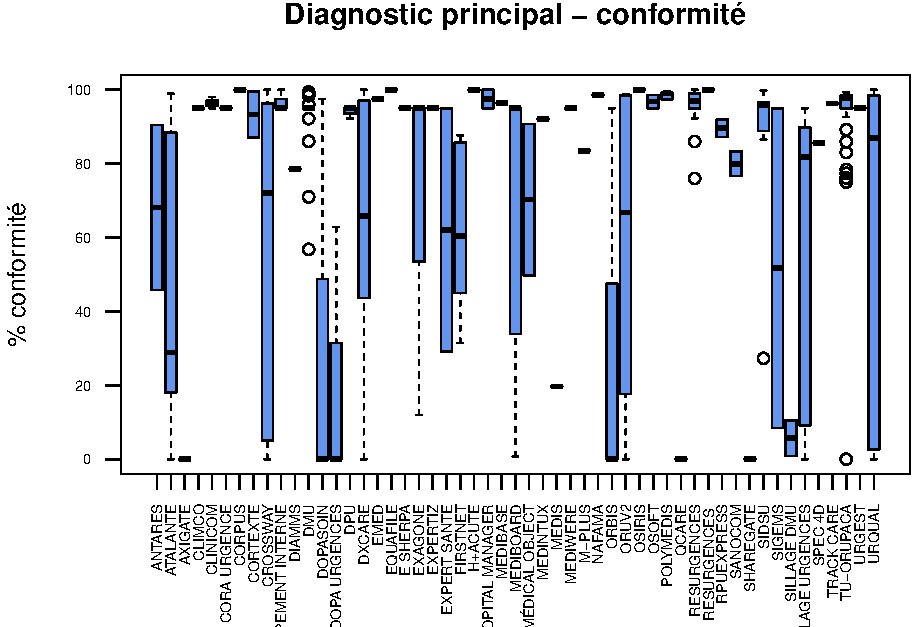
\includegraphics{septembre2015_files/figure-latex/unnamed-chunk-22-1.pdf}

\begin{itemize}
\itemsep1pt\parskip0pt\parsep0pt
\item
  taux de exhaustivité:
\end{itemize}

\begin{verbatim}
   Min. 1st Qu.  Median    Mean 3rd Qu.    Max.    NA's 
   0.00   95.10   99.80   87.72  100.00  100.00       7 
\end{verbatim}

\begin{itemize}
\itemsep1pt\parskip0pt\parsep0pt
\item
  exhaustivité par outil
\end{itemize}

\begin{verbatim}
                          Min    Max   moyenne  ecart-type Nb
AGFA EXAGON            100.00 100.00 100.00000          NA  1
ANTARES V2 DE INOVACUM  83.99  84.48  84.23500  0.34648232  2
ATALANTE                 0.00  99.14  59.77889 37.07903938  9
AXIGATE                100.00 100.00 100.00000          NA  1
CLIMCO                   0.00   0.00   0.00000          NA  1
CLINICOM                99.92 100.00  99.97333  0.04618802  3
CORA URGENCE            31.00  31.00  31.00000          NA  1
CORTEXTE                99.43  99.70  99.56500  0.19091883  2
CROSSWAY                 0.00  99.44  49.60273 47.97343850 12
DEVELOPPEMENT INTERNE  100.00 100.00 100.00000          NA  1
DIAMMS                  80.47  80.47  80.47000          NA  1
DMU                     97.41 100.00  99.80146  0.61222646 50
DOPASOIN                72.48 100.00  86.34000 13.76109007  3
DOPA URGENCES           69.10  82.60  77.36667  7.24315769  3
DPU                     99.76 100.00  99.92000  0.13856406  3
DXCARE                  21.05 100.00  86.85923 29.37125847 13
EMED                   100.00 100.00 100.00000          NA  1
E SHERPA               100.00 100.00 100.00000          NA  1
EXAGONE                  5.00 100.00  52.50000 67.17514421  2
EXPERTIZ                99.00 100.00  99.66667  0.57735027  3
EXPERT SANTE            81.00  81.00  81.00000          NA  1
EXPERT SANTÉ           100.00 100.00 100.00000          NA  1
HOPITAL MANAGER        100.00 100.00 100.00000  0.00000000  2
LOGICIEL MAISON         95.00 100.00  97.50000  3.53553391  2
MANUEL                  99.00  99.00  99.00000          NA  1
MEDIBASE                65.70  65.70  65.70000          NA  1
MEDIBOARD                2.00 100.00  84.92000 36.60915232  7
MÉDICAL OBJECT          49.76  90.69  70.22500 28.94188055  2
MEDINTUX               100.00 100.00 100.00000          NA  1
MEDIS                   13.50  13.50  13.50000          NA  1
MEDIWERE               100.00 100.00 100.00000          NA  1
M-PLUS                  16.80  16.80  16.80000          NA  1
NAFAMA                  99.80  99.80  99.80000          NA  1
ORBIS                   15.70  97.00  44.16667 45.80090974  5
ORUV2                   99.04 100.00  99.71000  0.44944410  4
OSIRIS                 100.00 100.00 100.00000          NA  1
OSOFT                  100.00 100.00 100.00000  0.00000000  2
POLYMEDIS               99.30  99.90  99.68000  0.26832816  5
QCARE                    0.00   0.00   0.00000          NA  1
RESURGENCES              0.00 100.00  78.62500 41.24861726 24
RPUEXPRESS              98.37  99.94  99.15500  1.11015765  2
SANOCOM                100.00 100.00 100.00000  0.00000000  2
SHAREGATE              100.00 100.00 100.00000  0.00000000  2
SIDSU                   98.20 100.00  99.45556  0.56593089  9
SIGEMS                  55.00  99.90  77.45000 31.74909448  3
SILLAGE DMU             98.80 100.00  99.40000  0.84852814  2
SILLAGE URGENCES        68.50  99.90  94.37500 10.77639616  8
SPEC 4D                 99.97  99.97  99.97000          NA  1
TRACK CARE              98.30  98.30  98.30000          NA  1
TU-ORUPACA               0.00 100.00  94.65756 15.66551586 45
URGEST                   0.00   0.00   0.00000          NA  1
URQUAL                   0.00 100.00  90.87000 22.09346414 35
\end{verbatim}

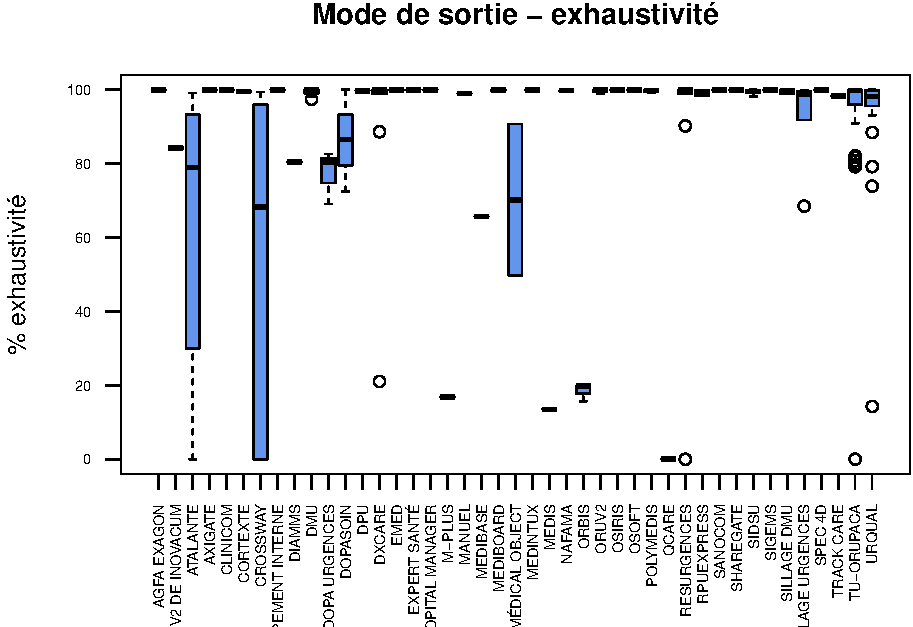
\includegraphics{septembre2015_files/figure-latex/unnamed-chunk-24-1.pdf}

\section{Conformité par région}\label{conformite-par-region}

\subsection{Date de naissance}\label{date-de-naissance-1}

\begin{verbatim}
                      Min Max   moyenne  ecart-type Nb
ALSACE             100.00 100 100.00000  0.00000000 18
AQUITAINE          100.00 100 100.00000  0.00000000 35
BOURGOGNE          100.00 100 100.00000  0.00000000 23
BRETAGNE            99.80 100  99.99167  0.03677362 30
CHAMPAGNE ARDENNES  99.80 100  99.98750  0.05000000 16
LIMOUSIN            99.95 100  99.99333  0.01658312  9
MIDI PYRENEES       98.74 100  99.95054  0.20698827 37
PACA                 0.00 100  97.99800 14.14185177 50
RHONE ALPES        100.00 100 100.00000  0.00000000 70
\end{verbatim}

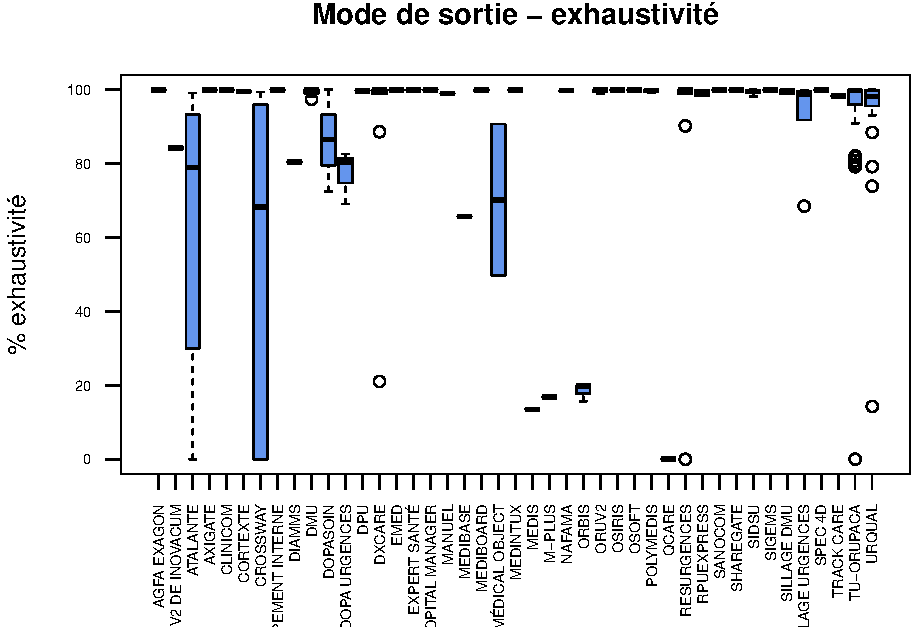
\includegraphics{septembre2015_files/figure-latex/unnamed-chunk-25-1.pdf}

\subsection{Diagnostic (DP)}\label{diagnostic-dp-1}

\begin{verbatim}
                     Min    Max  moyenne ecart-type Nb
ALSACE              0.00  98.95 52.12889  34.353078 18
AQUITAINE           0.00  99.80 63.42121  39.782563 35
BOURGOGNE           0.00 100.00 63.86957  44.685064 23
BRETAGNE            0.00 100.00 63.90567  40.977779 30
CHAMPAGNE ARDENNES  0.00  99.70 67.61875  41.100790 16
LIMOUSIN           85.57  98.98 96.81667   4.256727  9
MIDI PYRENEES       0.00 100.00 70.32676  37.940900 37
PACA                0.00  99.39 88.78780  23.584018 50
RHONE ALPES        95.00  95.00 95.00000   0.000000 70
\end{verbatim}

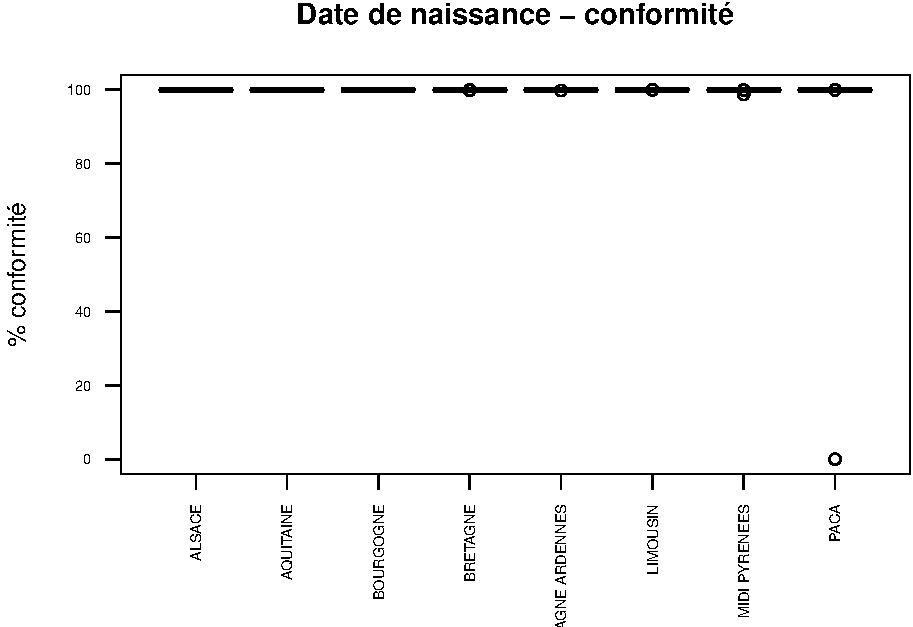
\includegraphics{septembre2015_files/figure-latex/unnamed-chunk-26-1.pdf}

\subsection{Mode de sortie (MS)}\label{mode-de-sortie-ms-1}

\begin{verbatim}
                     Min  Max  moyenne ecart-type Nb
ALSACE             15.70  100 68.77500 32.8245757 18
AQUITAINE           0.00  100 89.24242 27.5958220 35
BOURGOGNE           0.00  100 82.04348 38.5091232 23
BRETAGNE           13.50  100 91.54533 21.6244593 30
CHAMPAGNE ARDENNES 69.10  100 94.84375  9.6193533 16
LIMOUSIN           99.39  100 99.88667  0.2200568  9
MIDI PYRENEES       0.00  100 89.86405 20.8648135 37
PACA                0.00  100 87.24620 29.0773015 50
RHONE ALPES          Inf -Inf      NaN         NA 70
\end{verbatim}

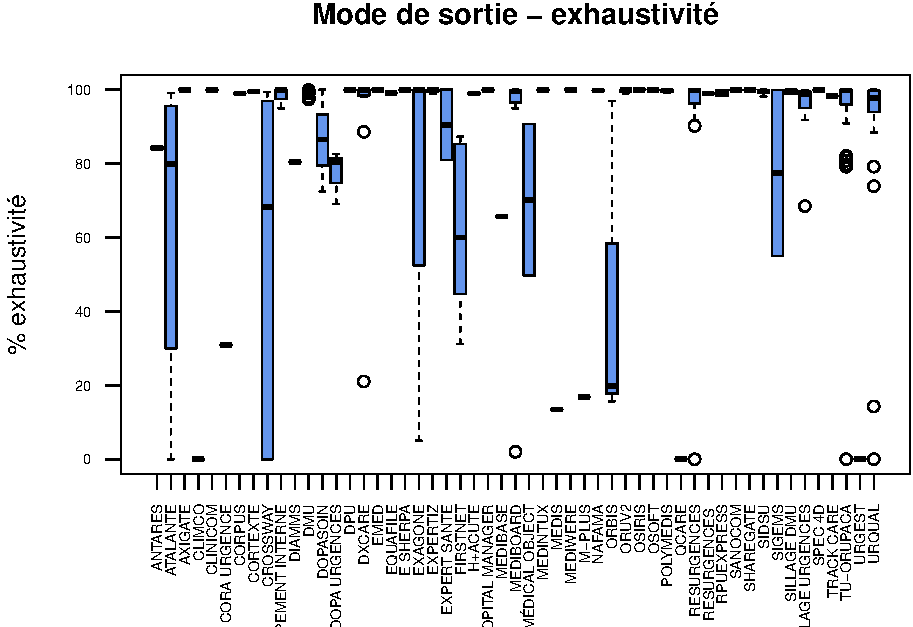
\includegraphics{septembre2015_files/figure-latex/unnamed-chunk-27-1.pdf}

\section{Exhaustivié par région}\label{exhaustivie-par-region}

\subsection{Date de naissance}\label{date-de-naissance-2}

\begin{verbatim}
                      Min Max   moyenne  ecart-type Nb
ALSACE             100.00 100 100.00000  0.00000000 18
AQUITAINE          100.00 100 100.00000  0.00000000 35
BOURGOGNE          100.00 100 100.00000  0.00000000 23
BRETAGNE           100.00 100 100.00000  0.00000000 30
CHAMPAGNE ARDENNES  99.80 100  99.98750  0.05000000 16
LIMOUSIN            99.95 100  99.99333  0.01658312  9
MIDI PYRENEES       99.96 100  99.99676  0.01028863 37
PACA                 0.00 100  97.99800 14.14185177 50
RHONE ALPES        100.00 100 100.00000  0.00000000 70
\end{verbatim}

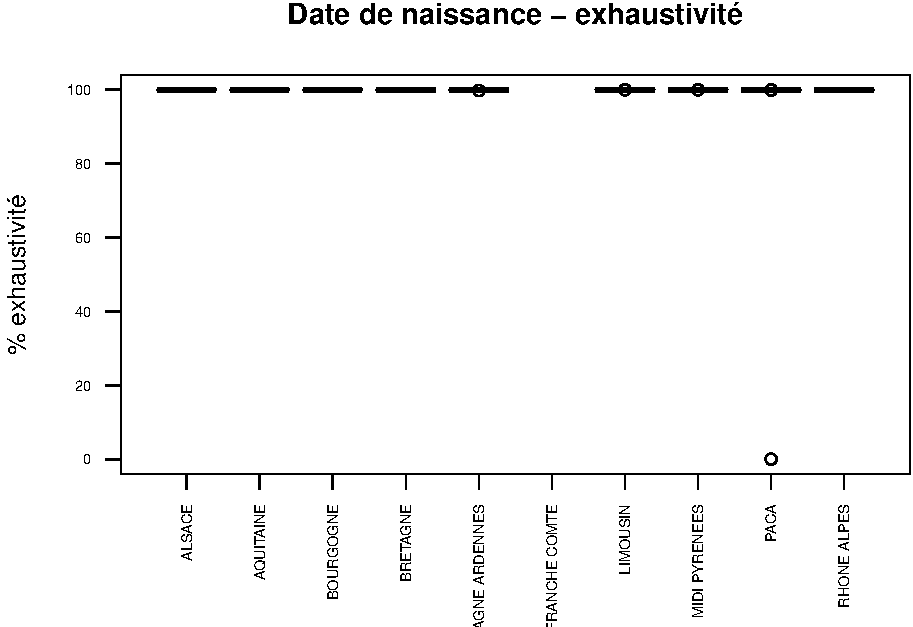
\includegraphics{septembre2015_files/figure-latex/unnamed-chunk-28-1.pdf}

\subsection{Diagnostic (DP)}\label{diagnostic-dp-2}

\begin{verbatim}
                     Min    Max  moyenne ecart-type Nb
ALSACE              0.00  98.95 52.12889  34.353078 18
AQUITAINE           0.00  99.80 63.42424  39.784993 35
BOURGOGNE           0.00 100.00 63.91304  44.720255 23
BRETAGNE            0.00 100.00 66.77667  39.331436 30
CHAMPAGNE ARDENNES  0.00  99.80 74.30625  37.783161 16
LIMOUSIN           85.57  98.98 96.81667   4.256727  9
MIDI PYRENEES       0.00 100.00 70.79919  38.082150 37
PACA                0.00 100.00 89.00340  23.627537 50
RHONE ALPES         0.00 100.00 72.23077  36.684793 70
\end{verbatim}

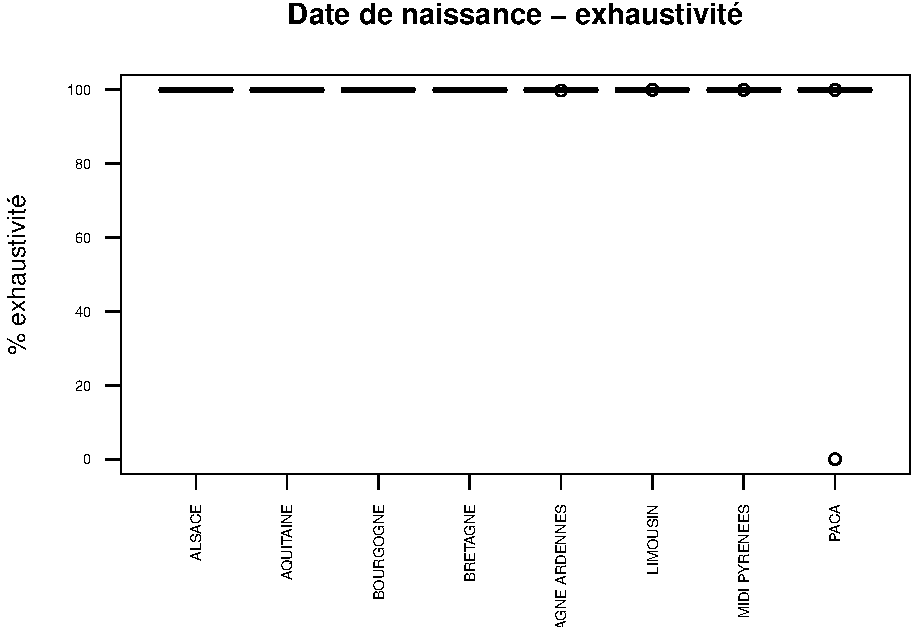
\includegraphics{septembre2015_files/figure-latex/unnamed-chunk-29-1.pdf}

\subsection{Mode de sortie (MS)}\label{mode-de-sortie-ms-2}

\begin{verbatim}
                     Min Max  moyenne ecart-type Nb
ALSACE             15.70 100 68.77500 32.8245757 18
AQUITAINE           0.00 100 89.24848 27.5976915 35
BOURGOGNE           0.00 100 82.04348 38.5091232 23
BRETAGNE           13.50 100 91.54533 21.6244593 30
CHAMPAGNE ARDENNES 69.10 100 94.84375  9.6193533 16
LIMOUSIN           99.39 100 99.88667  0.2200568  9
MIDI PYRENEES       0.00 100 92.50892 19.0664729 37
PACA                0.00 100 87.24620 29.0773015 50
RHONE ALPES         0.00 100 86.63077 31.7227093 70
\end{verbatim}

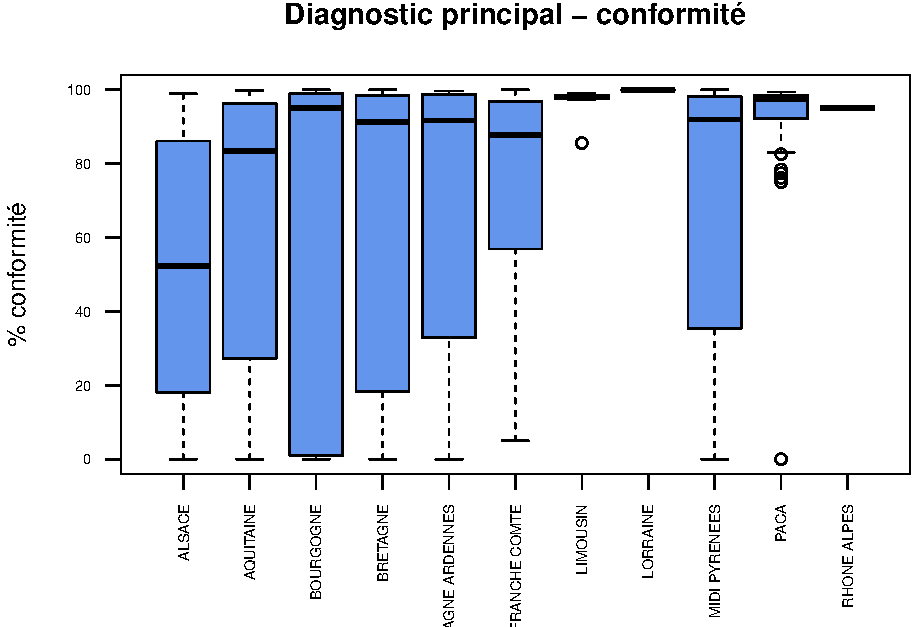
\includegraphics{septembre2015_files/figure-latex/unnamed-chunk-30-1.pdf}

\section{Résultats secondaires}\label{resultats-secondaires}

\subsection{\% de SU ne faisant pas de remontée de
RPU}\label{de-su-ne-faisant-pas-de-remontee-de-rpu}

\begin{verbatim}

 NON  OUI OUI  
  15  272    1 
\end{verbatim}

\begin{verbatim}
[1] "5.21 %"  "94.44 %" "0.35 %" 
\end{verbatim}

Messges pour les éditeurs, la DGOS, les DSI qui est responsable de quoi
? intégratin systématique des thésaurus, démarche d'amélioration.
Information proactive des sociétés savantes pour la publicationn des
Référentiels: info systématique de la Fedoru. Focaliser sur les
rectangles bleus. Voir si le n° de version permet de discriminer les
urqual qui remntent de ceux qui remontent mal.

\section{Analyse de Urqual}\label{analyse-de-urqual}

\end{document}
